%%%%%%%%%%%%%%%%%%%%%%%%%%%%%%%%%%%%%%%%%%%%%%%%%%%%%%%%%%%%%%%%%%%%%
%%%
%%% Set these variables appropriately
%%%
\newcommand{\AUTHORS}{Marcela Melara, Jenny Guo}
\newcommand{\TITLE}{BiscuitSpy: Profiling web users via HTTP cookies}
\newcommand{\KEYWORDS}{}
\newcommand{\CONFERENCE}{}
\newcommand{\PAGENUMBERS}{yes}       % "yes" or "no"
\newcommand{\TOAPPEAR}{no}
%%%
%%%
%%%%%%%%%%%%%%%%%%%%%%%%%%%%%%%%%%%%%%%%%%%%%%%%%%%%%%%%%%%%%%%%%%%%%

%%%% Setup the document/page
\documentclass[pdftex,twoside,12pt,letterpaper]{article}
\usepackage{ifthen}

\ifthenelse{\equal{\PAGENUMBERS}{yes}}{%
\usepackage[nohead,
            left=1in,right=1in,top=1in,
            footskip=0.5in,bottom=0.75in     % Room for page numbers
            ]{geometry}
}{%
\usepackage[noheadfoot,columnsep=0.2in,
            margin=1in,centering,truedimen]{geometry}
}

\usepackage{fancyhdr}
\usepackage[numbers,sort]{natbib}
\usepackage{xspace}
\usepackage{booktabs}
\usepackage{subfigure}
\usepackage[T1]{fontenc}
\usepackage{textcomp}
\usepackage{mathptmx}   % Times + Times-like math symbols
\usepackage{courier}
\usepackage[scaled=0.92]{helvet}

\usepackage{color}
\usepackage[pdftex]{graphicx}
\ifthenelse{\isundefined{\wantBW}}{%
  \usepackage[colorlinks]{hyperref}%        % for online version
}{%
  \usepackage[pdfborder={0 0 0}]{hyperref}% % for paper (B&W) version
}
\newcommand{\URL}[1]{\url{#1}}

%%%%% Setup for PDF
\hypersetup{%
pdfauthor = {\AUTHORS},
pdftitle = {\TITLE},
pdfsubject = {\CONFERENCE},
pdfkeywords = {\KEYWORDS},
bookmarksopen = {true}
}

%\setlength{\parindent}{0pt}
%\setlength{\parskip}{0pt}
\renewcommand{\headrulewidth}{0pt}
\newcommand{\Paragraph}[1]{\vspace{-2ex}\paragraph{#1.}}
\setlength{\topmargin}{-.15in}

\ifthenelse{\equal{\PAGENUMBERS}{yes}}{%
  \pagestyle{plain}
}{%
  \pagestyle{empty}
}

\makeatletter\long\def\@makecaption#1#2{
   \vskip 10pt
   \setbox\@tempboxa\hbox{\textsf{#1: #2}}
   \ifdim \wd\@tempboxa >\hsize % IF longer than one line:
       \textsf{#1: #2}\par      % THEN set as ordinary paragraph.
     \else                      % ELSE  center.
       \hbox to\hsize{\hfil\box\@tempboxa\hfil}
   \fi}
\makeatother

\clubpenalty=10000  % Don't allow orphans
\widowpenalty=10000 % Don't allow widows

\title{\textbf{\TITLE}}
\author{\AUTHORS}
\date{}

% Compact itemize and enumerate.  Note that they use the same counters and
% symbols as the usual itemize and enumerate environments.
\def\compactify{\itemsep=0pt \topsep=0pt \partopsep=0pt \parsep=0pt}
\let\latexusecounter=\usecounter
\newenvironment{CompactItemize}
  {\def\usecounter{\compactify\latexusecounter}
   \begin{itemize}}
  {\end{itemize}\let\usecounter=\latexusecounter}
\newenvironment{CompactEnumerate}
  {\def\usecounter{\compactify\latexusecounter}
   \begin{enumerate}}
  {\end{enumerate}\let\usecounter=\latexusecounter}

\newcommand{\comment}[1]{\textcolor{red}{#1}}
\newcommand{\ignore}[1]{}

\newcommand{\xc}[1]{\mbox{\textit{#1}}}
\newcommand{\la}{\leftarrow}
\newcommand{\ra}{\rightarrow}
\newcommand{\somespace}{\hspace{0.1cm}}

\def\discretionaryslash{\discretionary{/}{}{/}}
\def\discretionarydot{\discretionary{.}{}{.}}
\def\discretionarycolon{\discretionary{:}{}{:}}
{\catcode`\/\active
\catcode`\.\active
\catcode`\:\active
\gdef\URLprepare{\catcode`\/\active\let/\discretionaryslash
                 \catcode`\.\active\let.\discretionarydot
                 \catcode`\:\active\let:\discretionarycolon
        \def~{\char`\~}}}%
\def\URL{\bgroup\URLprepare\realURL}%
\def\realURL#1{\tt #1\egroup}%

\newcommand{\eg}{{\em e.g.}, }
\newcommand{\ie}{{\em i.e.}, }
\newcommand{\etal}{{\em et al.\ }}

\def\check{\stackrel{{\scriptscriptstyle ?}}{=}}

\begin{document}
\maketitle

\section{Introduction}
\label{sec:intro}

HTTP cookies were originally introduced as a mechanism to make websites stateful \cite{httpcookies}.
Websites use these small pieces of data to keep track of a user's browsing activity, such as whether she is logged in, or which items she has added to her shopping cart, and they store these cookies on the client-side in the user's web browser \cite{httpcookies}.
When the user loads the website, the browser will send the appropriate stored cookies back to the web server to return to the last recorded state.
However, HTTP cookies are not only being used to improve the user online experience.
Because cookies allow websites to remember a given user's browsing activity or preferences on that site, online advertising companies have found a way to leverage HTTP cookies and take advantage of the vast amounts of available user information online.
At the same time, website publishers themselves now often employ \emph{analytics cookies}, special HTTP cookies used collect statistics about their users and the usage of their website.

In addition to the cookies required for the functionality of a website, advertising companies include \emph{tracking cookies} and website publishers add analytics cookies when a user visits this site.
Such cookies have been raising concerns about users' privacy online since they were first observed \textbf{(citation needed)} because companies can compile a vast browsing history for users and learn about their personal preferences and habits \cite{dntbill}.
Moreover, researchers have found that cookies may 
\section{Background}
\label{sec:background}

% I think this section should include an explanation of the types of cookies we looked for when searching for profiling cookies
Global cookies, such as DoubleClick's \texttt{id} cookie, have a globally unique value, \emph{i.e.,} its value remains the same across different visited websites in each \emph{session} (\textbf{NEEDS VERIFICATION: per session, or per lifetime}. 
Ad companies use these cookies to track user through their web and collect information about their browsing habits and personal preferences.

Local cookies, on the other hand, such as the Google Analytics \texttt{\_\_utma} cookie, have locally unique values.
This means that each unique domain that utilizes such a cookie to track an individual user will have a unique user identifier for the entire \emph{lifetime} of the cookie (\textbf{NEEDS VERIFICATION: per session, or per lifetime}.
These kinds of cookies are used by domains to keep track of their own users and their browsing habits pertaining to their website. 

\subsection{Cookies used by Google}
As Google cookies are one of the most pervasive cookies on the Internet we start by giving an overview of the different types of cookies that Google uses. They can be divided into the following categories:

\subsubsection{Preferences}
Preference cookies allow Google to keep track of user preferences in order to provide a more personalized browsing experience. Information stored include default language, user region, number of search results to display per page, text size and font and other preferences. Notably through the use of these cookies, Google does not require the user to be signed in to provide the targeted Google website. The PREF cookie is the most dominant cookie for storing user preferences. It also includes a timestamp of the most recent user preference change. This unique information can be used to pinpoint individual users due to the unlikelihood that two users have the same timestamp.

\subsubsection{Security}
Security cookies are used to authenticate users and prevent fraudulent use of login credentials. They store the Google account ID and most recent sign-in time in an encrypted and signed string. Security cookie names end with SID, such as SID, HSID, SAPISID and APISID. The APISID cookie and SAPISID cookie both contain two encrypted strings, where the second string is \emph{unique across all Google websites and per cookie lifetime}. Therefore, despite the encryption, it is still possible to identify individual users and profile what Google services the user is visiting.

\subsubsection{Processes}
Process cookies support the display and function of more complex and dynamic websites. Google states that these cookies are necessary for the proper functioning of some websites. (\textbf{REFERENCE}) For example blooking an 'lbcs' cookie would prevent Google docs from opening documents correctly. BiscuitSpy does not include this cookie in its profiling.

\subsubsection{Advertising}
Advertising cookies are used to determine which ads to display to the user and for tracking the user's ad clicking behavior through a complex network of publishers, advertisers and website operators. The most commonly seen advertising cookie is the 'id' cookie from the domain ad.doubleclick.net. The second field of the 'id' cookie contains several numbers that remain the same during multiple visits of the same website, but change their values either when the user has clicked on an advertisement on the website, or when the website displays a different ad. It can thus be inferred that the numbers encode the ads to display and whether the user has clicked on them.

\subsubsection{Session State}
Session state cookies collect information about how users interact with a website and keep information of the previous sessions of a website. Youtube session cookies for example store a list of most recent videos watched in that browser. Session state cookies are also used to measure the effectiveness of affiliate advertising. It is difficult to determine the exact names of session cookies and the meaning of their values, therefore BiscuitSpy currently does not leverage session cookies for user profiling.

\subsubsection{Analytics}
Analytics cookies represent the largest group of Google cookies and are mainly used by BiscuitSpy to gather user profile information. While the previous cookies all belong to a Google domain, analytics cookies do not have that restriction and can be found on all websites that use Google Analytics (GA) and are stored under the current website's domain. The five main cookies set by GA are  \_utma,  \_utmb, \_utmc, \_utmv and \_utmz. 

\begin{figure}[h]
\centering
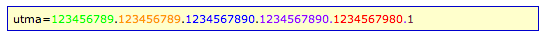
\includegraphics[scale=0.8]{./diagrams/utma.png}

\begin{tabular}{ | l | p{12cm} |}
    \hline
  Cookie Field & Description \\ \hline
Domain Hash & The first number is the domain hash. This is set by all cookies from this domain. \\ \hline
Visitor ID & The second number is a random "unique ID". \\ \hline
Initial visit & The third number is the unix time stamp for the initial visit and is set as soon as you enter the site. \\ \hline
Previous Session & The third number is the unix time stamp for the previous session. \\ \hline
Current Session & The fourth nubmer is the unix time stamp for the current session. \\ \hline
Session number & Contains the number of visits to this website since cookie creation. \\ \hline
 \end{tabular}

\caption{Google Analytics UTMA cookie}
\label{fig:utma}

\end{figure}

As an example, Figure \ref{fig:utma} shows the individual components of the \_utma cookie. The timestamp information of the initial, most recent and current visit in combination with the number of visits to the website allow for an accurate reconstruction of user's browsing behavior. 
\\
\\
For the BiscuitSpy implementation we leveraged preference cookies, advertising cookies and analytics cookies. We did not filter out process cookies and session state cookies, since we were unable to identify the specific cookie names and individual cookie field meanings.


\subsection{Common third-party cookies}
While Google cookies are the most common cookies found on websites, we also identified several other common third-party cookies from amazon, facebook and twitter.

A common Amazon third party cookie is the \texttt{apn-user-id} cookie. This cookie contains the user-id as shared by the amazon partner's network. The most common Facebook third party cookie is the \texttt{datr} cookie. This cookie encodes a user id and remains the same across websites and browsing sessions. Twitter's third party cookie is the \texttt{guest\_id} cookie which contains a version number and an encoded user id. It is interesting to see how these other non-google cookies become more and more prevalent on the web and challenge Google's position as the dominent user and ad tracking cookie provider.






\section{Design}
\label{sec:design}





\section{Evaluation}
\label{sec:eval}

% Jenny, feel free to modify this as you see fit
We tested our BiscuitSpy prototype on the an open home wireless LAN with MAC Address filtering as well as on the open Princeton University WiFi network, which also has MAC Address filtering. Due to factory configuration issues, we were never able to capture useful packets from devices on either network. However, we deem our current prototype sufficient for demonstrating the feasibility of profiling a user based on HTTP cookies.
\section{Related Work}
\label{sec:related}


\section{Future Work}
\label{sec:future}

Example of incorporation citations~\cite{coral:nsdi04}.


\section{Conclusion}
\label{sec:conclusion}

BiscuitSpy was built as a proof-of-concept software for profiling web users based on http cookies. It offers functionality to capture packets on an open wireless network and filter out http headers which transmit cookie data. The captured cookie data is combined with existing cookie definitions to extract relevant user information. In our work we showed that captured cookies leak various personal information, such as browsing behavior, location information, username and e-mail address and unique brower identifiers. By aggregating the cookie information from multiple sources, BiscuitSpy can built up a comprehensive user profile.

%% Bibliography
%\vspace{-1ex}
%\linespread{1.0}
%\setlength{\bibsep}{1pt}
%\footnotesize
\small
\bibliography{local}
\bibliographystyle{abbrvnat}

\end{document}

